\documentclass[12pt,a4paper]{article}

\usepackage[english,italian]{babel}
\usepackage[T1]{fontenc}

\usepackage[margin=2cm]{geometry} %margini
\usepackage{float} %float per immagini e tabelle
\usepackage{graphicx} %figure
%\usepackage{minted}

\setcounter{secnumdepth}{4}

%\newcommand{\htmlcode}[1]{\mintinline{html}{#1}}
%\newcommand{\csscode}[1]{\mintinline{css}{#1}}
%\newcommand{\jscode}[1]{\mintinline{js}{#1}}
%\newcommand{\phpcode}[1]{\mintinline{php}{#1}}
%\newcommand{\sqlcode}[1]{\mintinline{sql}{#1}}

\usepackage{hyperref}

\title{Progetto di Tecnologie Web}
\date{Anno accademico 2020/2021}

\begin{document}
\pagenumbering{gobble}
\maketitle
\begin{figure}[H]
	\centering
	
\includegraphics[width=4cm]{img/unipd.png}
\end{figure}
\begin{figure}[H]
	\centering
	
\includegraphics[width=8cm]{img/logo.png}
\end{figure}
\begin{table}[H]
	\centering
	\begin{tabular}{c|c c c}
		\textbf{Componenti} & Kostadinov     & Samuel  & 1187605 \\
		                    & Roveroni       & Emma    & 1187275 \\
		                    & Tesser         & Marco   & 1201154 \\
		                    & Uderzo         & Marco   & 1201290 \\
	\end{tabular}
\end{table}

\begin{center}
	\textbf{Indirizzo sito web}: http://tecweb2021.studenti.math.unipd.it/mtesser\\
	\textbf{Email referente del gruppo}: samuel.kostadinov@studenti.unipd.it
\end{center}

\begin{table}[H]
	\centering
	\begin{tabular}{c|c c}
		\textbf{Utenti} & \textbf{Nickname} & \textbf{Password} \\
		\hline
		Admin           & admin        			& admin        \\
		User            & user         			& user         \\
		Utente 1        & MarcoTesser 			& MarcoT       \\
		Utente 2        & MarcoUderzo  			& MarcoU       \\
		Utente 3        & EmmaRoveroni 			& EmmaR        \\
		Utente 4        & SamuelKostadinov  	& SamuelK      \\

	\end{tabular}
\end{table}
\newpage
\pagenumbering{roman}
\tableofcontents
\newpage
\pagenumbering{arabic}
\renewcommand{\abstractname}{Abstract}
\begin{abstract}
	\emph{Physique} è un sito incentrato sul fitness che permette a tutti i suoi utenti, siano essi neofiti o esperti, di ricevere consigli legati al mondo dell'attività fisica in palestra e di interagire tra loro tramite un forum. \newline
	Il sito offre la possibilità di vedere alcuni esempi di allenamenti per tutti, alcune ricette sane che permettono di mantenere la linea e le news riguardanti il mondo del fitness. 
\end{abstract}
\newpage
\section{Fase di analisi}
\subsection{Analisi delle caratteristiche dell'utenza}
\label{sub:analisi_delle_caratteristiche_dell_utenza}
\subsubsection{Destinatari}
\label{subs:destinatari}
Il sito \emph{Physique} si rivolge sia a chi è alle prime armi nel mondo del fitness, sia a chi è un atleta esperto che vuole far parte di una community e condividere i suoi risultati. 
L'interfaccia si propone di essere il più semplice e intuitiva possibile per facilitare tutti gli utenti nella fruizione del sito stesso. I tipi di utenti individuati sono:
\begin{itemize}
    \item l'\textit{utente generico}, che non è registrato al sito o non ha effettuato il login;
    \item l'\textit{utente registrato}, che ha effettuato il login;
    \item l'\textit{utente amministratore}, che possiede privilegi rispetto agli altri utenti.
\end{itemize}

\subsubsection{Funzionalità}
\label{subs:funzionalità}
Qualsiasi tipo di utente può navigare all'interno del sito, visualizzare tutti gli allenamenti descritti, le ricette e le news presenti e prendere visione dei post presenti nel forum.\\
L'utente generico può creare un proprio account tramite la funzionalità di signup. L'utente registrato potrà accedere al proprio account ogni volta che lo desidera. Una volta effettuato l'accesso, l'utente potrà:
\begin{itemize}
    \item visualizzare la propria pagina utente;
    \item modificare i propri dati;
    \item inserire post nel forum o risposte al post di qualcun altro;
    \item lasciare mi piace ai post degli altri utenti.
\end{itemize}
L'utente amministratore, oltre a possedere tutte le funzionalità degli altri utenti, può:
\begin{itemize}
	\item aggiungere ed eliminare ricette.
	\item aggiungere ed eliminare news.
	\item eliminare post o risposte ai post.
	\item promuovere un utente al grado di amministratore.
	\item bannare o revocare il ban di un utente.
	\item eliminare l'account di un utente.
\end{itemize}


\newpage
\section{Fase di progettazione}
\subsection{Progettazione}
In una prima fase, il gruppo si è riunito per decidere il tema del sito web da sviluppare. Sono state raccolte le varie idee, decise le funzionalità e gli obiettivi da raggiungere, quali tipologie di argomenti trattare in ciascuna pagina, impostato il layout del sito e decisi i colori da utilizzare. Inoltre sono state decise le tecnologie da usare e si è decisa una prima suddivisione dei compiti individuali. \\
Successivamente è stato progettato il database, nel quale vengono immagazzinate e organizzate le informazioni relative agli utenti e ai contenuti pubblicati sul sito web. Allo stesso tempo, è stato portato avanti lo sviluppo della parte front end del sito, prestando particolare attenzione anche all'accessibilità e alla visualizzazione del sito su dispositivi di diverse dimensioni. \\
Infine, il sito è stato approfonditamente testato al fine di rilevare e risolvere eventuali bug e di validare la compatibilità con i differenti browser e dispositivi.
\subsection{Struttura}
\subsubsection{Header}
L'header contiene il logo, il titolo della pagina su cui ci si trova e due link, uno per il login e l'altro per il signup. Questi ultimi due link sono visibili solo nel caso in cui l'utente non abbia ancora effettuato l'accesso. Dopo che l'utente ha eseguito l'accesso, al posto dei due link login e signup, sarà presente un solo link, ovvero quello per il logout, il quale, una volta cliccato, scollegherà l'utente. 
\subsubsection{Breadcrumb}
Lo scopo del breadcrumb è quello di indicare all'utente dove si trova all'interno del sito e il percorso per arrivare in tale pagina, in modo che gli sia più facile orientarsi durante la navigazione all'interno del sito e che possa facilmente tornare indietro. L'ultimo campo corrisponde alla pagina corrente e, per evitare link circolari, questo non è cliccabile.
\subsubsection{Container}
La classe container comprende il menù e il contenuto del sito.
\paragraph{Menù}
Il menù è posizionato sulla sinstra e contiene tutte le pagine raggiungibili tramite il sito:
\begin{itemize}
	\item \textit{Home};
	\item \textit{Workout};
	\item \textit{Alimentazione};
	\item \textit{Forum};
	\item \textit{News}.
\end{itemize}
Nel caso in cui l'utente abbia effettuato l'accesso, nel menù sarà presente anche il link alla pagina \textit{Profilo}. Se l'utente è un amministratore verrà visualizzato anche il link per il \textit{Pannello admin}.
\paragraph{Content}
Lo scopo di content è quello di esporre i contenuti proposti dal sito.
\subparagraph{Home}
La pagina home è quella principale, ovvero la prima che si vede quando si visita il sito. Al suo interno sono presenti una descrizione del sito, le funzionalità che possono essere trovate all'interno del sito ed infine la foto del team.
\subparagraph{Workout}
La pagina workout espone i concetti basilari ed imprescindibili della programmazione dell'allenamento. É perciò rivolta al principiante che ha intenzione di entrare in palestra per la prima volta, o che si è finora allenato in modo non ottimale.
La pagina è suddivisa in paragrafi che danno un'introduzione al motivo per cui è da preferire una programmazione di allenamento studiata.
In fondo alla pagina si possono trovare dei link che rimandano alle principali tipologie di suddivisione dell'allenamento.
\subparagraph{Split}
Le pagine split sono 4:
\begin{itemize}
\item Bro Split;
\item Push-Pull-Legs;
\item Upper-Lower;
\item Full-Body;
\end{itemize}           
Tutte e 4 hanno una struttura simile tra di loro.
Sono suddivise in paragrafi in cui viene spiegato in cosa consiste lo split, per poi elencare i suoi vantaggi e svantaggi ed infine mostrarne un esempio in forma tabellare.
In tutte le pagine è presente un link \textit{Indietro} che riporta alla pagina workout principale. 
\subparagraph{Alimentazione}
La pagina di alimentazione contiene un elenco di ricette, che sono presentate in riquadri contenenti il nome della ricetta, l’immagine
del piatto, una breve descrizione del piatto ed infine il link che apre la pagina completa della ricetta. 
\subparagraph{Ricetta}
La pagina della ricetta completa riporta il titolo della stessa seguito da una foto del risultato finale del piatto. Successivamente vengono elencati gli ingredienti necessari alla preparazione, viene illustrato il procedimento da seguire ed, eventualmente, vengono dati dei consigli per agevolare la riuscita della ricetta. In tutte le pagine è presente un link \textit{Indietro} che riporta alla pagina alimentazione principale.
\subparagraph{Forum}
La pagina del forum, nel caso in cui l'utente non abbia effettuato l'accesso, chiederà all'utente di accedere o registrarsi per lasciare commenti. Nel caso in cui questo non avvenga l'utente avrà solo la possibilità di leggere i post ed i commenti lasciati dagli altri utenti e non potrà interagire con il forum in alcun modo.
Al contrario, nel caso in cui l'utente abbia effettuato l'accesso, per primo verrà visualizzato un form per lasciare un commento e sotto, come nel caso precedente, l'elenco di tutti i post con ora anche la possibilità di lasciare eventualmente un like e di rispondere a questi.
\subparagraph{News}
La pagina delle news riporta, al primo accesso, una lista con tutte le notizie del sito di ogni categoria. Queste, successivamente potranno essere filtrate, e quindi ci sarà la possibilità di visualizzare solo le news relative a: workout, alimentazione o notizie del sito.
\subparagraph{Profilo}
La pagina del profilo permette all'utente di visualizzare e modificare alcune informazioni relative al suo account come: nome, cognome, email e password.
\subparagraph{Pannello admin}
La pagina del pannello admin permette all'amministratore di effettuare delle modifiche, rimozioni od inserimenti all'interno del sito, tra cui: 
\begin{itemize}
	\item promuovere un utente da standard ad amministratore;
	\item eliminare ricette, news, post ed eventualmente relative risposte;
	\item aggiungere news e ricette;
	\item bannare un utente dal forum, rimuovere il ban;
	\item rimuovere anche degli account;
\end{itemize}     
\subparagraph{Signup e login}
Le pagine di signup e login permettono all'utente rispettivamente di  registrarsi o accedere con le proprie credenziali al sito. Nella pagina signup sono presenti dei campi per inserire username, indirizzo email, nome, cognome e la password (quest’ultima da inserire due volte per confermare la correttezza). Per il login invece è necessario solamente inserire l'username e la password.
\subsection{Visualizzazione}
Il sito è stato pensato in modo da avere una visualizzazione adatta ad ogni tipologia di dispositivo ed in modo da avere pagine accessibili ad una categoria di utenti più ampia possibile.
Sono state quindi realizzate tre tipologie di visualizzazione del sito: desktop, mobile e stampa.
\paragraph{Desktop}
Nella visualizzazione desktop il layout è diviso in 4 sezioni.
La prima sezione, ossia l'header,contiene al suo interno: il logo del sito,il nome della pagina in cui ci si trova ed infine le opzioni di autenticazione(login e signup se non si è effettuato l'accesso e logout nel caso contrario).
La seconda sezione, ossia il breadcrumb,contiene il percorso effettuato per arrivare alla pagina corrente.
La terza sezione, ossia il menu,elenca le pagine principali del sito.
La quarta sezione, ossia il content, racchiude il contenuto che si adatta in base alla grandezza della schermata.
\paragraph{Mobile}
Nella visualizzazione mobile è stato implementato il menù ad hamburger al fine di gestire al meglio lo spazio disponibile. Questo compare all'interno del breadcrumb, a destra, e per espanderlo è necessario cliccare sull'icona. Una volta espanso, il menù si sviluppa in verticale. Per chiuderlo, bisogna cliccare sul simbolo di "\textit{X}" che si trova al posto dell'icona del menù. \\
Il resto delle pagine ha il medesimo layout della versione desktop, fanno eccezione le tabelle presenti nelle singole pagine \textit{Split}. Infatti, per realizzare le tabelle nella visualizzazione mobile è stato seguito l'approccio \textit{Responsive table}. 
%mettere foto tabella e menù con media query
\paragraph{Stampa}
Per quanto riguarda la stampa, sono stati tenuti solo gli elementi fondamentali, ovvero il contenuto della pagina, tralasciando, quindi, gli elementi di presentazione (immagini e
background). È stato rimosso il menù, il logo del sito, perché non necessari, mentre è stato mantenuto il breadcrumb, per specificare il percorso alla pagina corrente. Le pagine sono in bianco e nero per
enfatizzare il contenuto anziché la presentazione, è stato rimosso il bordo nei titoli dei paragrafi e per i link che portano al di fuori del sito ne è stata aggiunta la versione completa. Infine, il font, che nella visualizzazione a schermo era sans-serif,  è diventato serif per una migliore leggibilità su carta stampata.

\subsection{Accessibilità}
Si sono seguite le linee guida del WCAG in modo da sviluppare un sito web che abbia un alto livello di accessibilità. Fondamentale è stata la suddivisione fra contenuto, presentazione e comportamento, che garantisce un buon posizionamento nei motori di ricerca e una buona interazione con gli utenti che presentano disabilità visive.

\subsubsection{Contenuto}
Il breadcrumb, presente in ciascuna pagina, permette all'utente di sapere in ogni momento dove si trova all'interno del sito e il percorso che ha fatto per raggiungere tale pagina. Per evitare link circolari, l'ultimo campo del breadcrumb (che corrisponde alla pagina corrente) e la voce del menù della pagina corrente, non sono cliccabili. L'utente può conoscere quale altre pagine può raggiungere da quella in cui si trova perchè i link che si trovano all'interno di questa sono sottolineati. 
Per aiutare gli utenti che utilizzano lo screen reader, è presente un link nascosto che gli permette di andare direttamente al contenuto della pagina corrente, saltando il menù. Inoltre per ogni immagine, incapsulate nel tag \textit{img}, è presente il tag \textit{alt}  che fornisce una  descrizione alternativa per gli screen reader. 
All'interno del sito si trovano parole in lingua straniera le quali sono accompagnate dal tag span che ne specifica tramite \textit{xml:lang="..."} la lingua della parola in questione. 


\subsubsection{Presentazione}
Il design del sito è stato implementato, tramite CSS, usando classi che definiscono il contenuto
dell’oggetto e non il comportamento, in modo da mantenere la separazione tra comportamento e presentazione. É presente un foglio di stile unico in cui si trova il codice dedicato alla visualizzazione desktop, stampa e mobile. Questi ultimi due sono stati effettuati tramite \textit{media query}. Vengono usate principalmente misure relative (em) o in percentuale per permettere una corretta visualizzazione delle pagine su schermi di dimensioni diverse. 
Il colore principale del sito è l'azzurro, che contrasta le scritte, per esempio dei titoli, i quali sono in bianco. Per distinguere i link già visitati, si è deciso di evidenziare quest'ultimi con il colore viola, mentre i link non ancora visitati richiamano il colore che domina il sito, cioè l'azzurro. 


\subsubsection{Comportamento}
Le informazioni all'interno del sito sono reperibili con un numero
limitato di click, infatti la maggior parte delle informazioni sono raggiungibili tramite il menù. 
Per facilitare la navigazione, le pagine che possono portare ad altre pagine, come workout e alimentazione, presentano, all'inizio della pagina, il link \textit{Indietro} che riporta l'utente alla pagina principale della relativa sezione. 
I dati inseriti in input dall'utente sono stati validati per garantirne il corretto inserimento. Nel caso un input non superi la validazione, viene mostrato un messaggio d'errore, contenente la spiegazione dell’errore commesso.


\newpage
\section{Fase di implementazione}
\subsection{Linguaggi}
\subsubsection{HTML}
Il linguaggio di markup scelto per realizzare tutte le pagine del sito è XHTML. Si è preferito questo a HTML5 per i seguenti motivi:
\begin{itemize}
    \item garantisce alta compatibilità con i browser più obsoleti;
    \item i tag <html>, <head>, <title> e <body> sono obbligatori;
	\item gli elementi devono essere nidificati correttamente;
	\item gli elementi devono essere sempre chiusi;
	\item gli elementi devono essere sempre in minuscolo;
	\item i nomi degli attributi devono essere sempre in minuscolo.
\end{itemize}

Per le form di registrazione e accesso, abbiamo scelto di utilizzare come input per le e-mail il tipo text che, grazie ad opportuni controlli specificati nella sezione \S\ref{subs:php}, 
si comporta similmente al tipo email di HTML5.
%non so cosa dire

\subsubsection{CSS}
Per la realizzazione del design del sito è stato adottato CSS3. 
Con lo scopo di garantire la corretta separazione fra contenuto e presentazione, è stato usato un foglio di stile esterno anziché ricorrere ai tag di stile all'interno del codice XHTML. 
Come unità di misura si è scelto di utilizzare quelle relative per la loro adattabilità.
%non so cos'altro scrivere
\subsubsection{SQL}

Il database contiene le informazioni di tutte le pagine costruite dinamicamente, ovvero \textit{Alimentazione}, \textit{News} e \textit{Forum}. É inoltre presente una tabella con tutti gli utenti del sito e i relativi dati.\\
Le chiavi delle tabelle sono nella quasi totalità dei casi degli indici autoincrementali, tranne nel caso di utente che ha come chiave primaria lo username (chiamato \textit{IDUtente} nella tabella) e nel caso di \textit{likes}, 
in cui la chiave primaria è la combinazione di utente e id del post a cui è stato messo il like.

Lo schema relazionale del database è il seguente: 

\begin{figure}
	\centering
	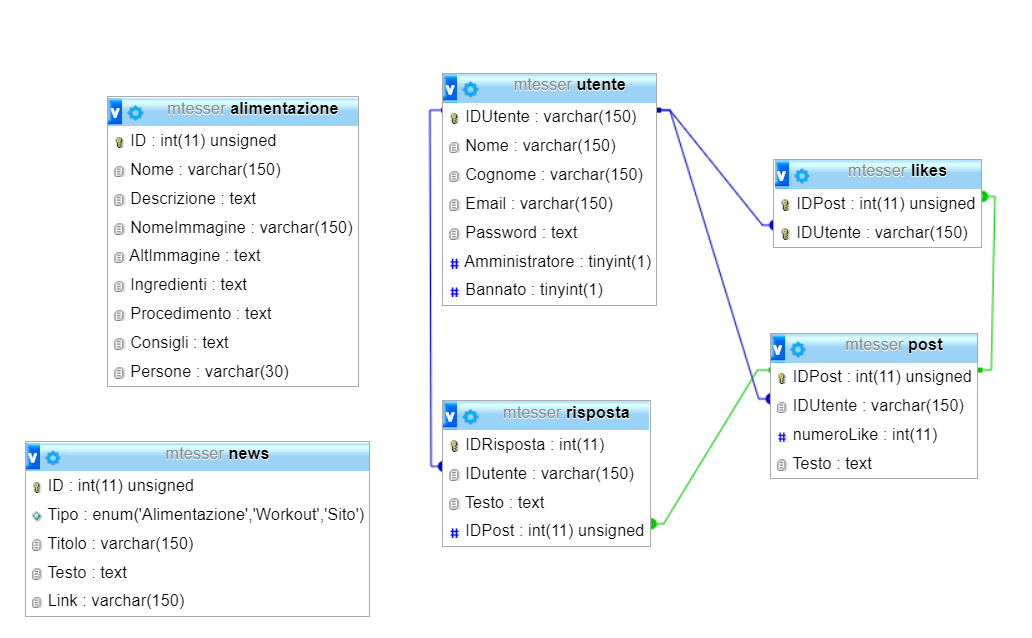
\includegraphics[width=18cm]{img/database.png}
\end{figure}
\newpage
Al fine di evitare problematiche causate dall'eliminazione dei post, quando uno di questi viene cancellato, vengono rimosse anche tutte le risposte e tutti i like. Allo stesso modo vengono eliminati anche tutti i post, 
tutti i like e tutte le risposte quando un utente viene eliminato.

\subsubsection{PHP}\label{subs:php}

Tutte le pagine del sito sono costruite dinamicamente, nella maggior parte dei casi utilizzando solamente il linguaggio PHP.\\
Ogni pagina ha un template, riconoscibile tra i file .xhtml in quanto contiene la parola \textit{base} nel nome. Ci sono 4 template nel progetto:

\begin{itemize}
    
	\item adminBase.xhtml
    \item profileBase.xhtml
	\item forumBase.xhtml
	\item base.xhtml
	
\end{itemize}

La differenza tra le varie pagine che ci ha portati a definire 4 template sono gli script Javascript che dovevano essere inclusi soltanto in alcune pagine. Queste pagine contengono la struttura base dei div, 
i quali fungono da contenitori per tutti gli elementi del sito, e che vengono costruiti dinamicamente. Tramite alcuni tag vuoti non validi riusciamo infatti a sostituire i contenuti della pagina molto velocemente tramite i parametri \textit{get}.\\

Il cuore di questo sistema sono le due classi PHP \textit{Renderer} e \textit{Parser}, che permettono di creare i contenuti delle varie pagine in base al parametro \textit{get 'r'} e ad una serie di convenzioni utilizzate per i tag vuoti. La classe Parser, infatti,
tiene in un campo privato tutte le possibili route indicate nel file index.php, una funzione e un array di variabili per ogni route. Nel file index.php alla fine viene chiamata la funzione \textit{parse}, che, se il parametro \textit{get 'r'} esiste ed è presente nel campo apposito 
del parser, renderizza il file corrispondente (tramite la classe Renderer, spiegata nel paragrafo successivo) e chiama una funzione passata durante il setup fatto in index.php. Questo permette di creare dinamicamente i contenuti utilizzando i file .xhtml.
La classe Renderer si occupa di renderizzare i file in base ai diversi tipi di placeholder, ovvero i tag vuoti, e i vari simboli speciali tramite delle funzioni di utility. 
I vari tipi di placeholder sono 4:

\begin{itemize}
    
	\item includePlaceholder
    \item blockPlaceholder
	\item ifPlaceholder
	\item variablePlaceholder
	
\end{itemize}

Ognuno di questi placeholder ha un preciso significato, riportato di seguito:

\begin{itemize}
    
	\item includePlaceholder: questo placeholder, obbligatorio, identifica una base alla pagina corrente. Si trova all'inizio della pagina e ha la forma <includeBasePlaceholder />. Il Renderer, quando trova un tag in questa forma, tramite un'espressione regolare prende il file con il nome corrispondente alla sottostringa compresa tra include e Placeholder e ne inserisce i contenuti nella pagina;
	
    \item blockPlaceholder: questo placeholder ha la forma <blockSetBlocknamePlaceholder /> e si trova in tutte le pagine. Questo placeholder indica che in quel particolare punto della pagina va inserito un blocco di codice html. Il blocco è identificato dal 
	nome, ovvero la sottostringa compresa tra Set e Placeholder. L'identificativo è infatti usato nella sostituzione del tag vuoto, in quanto il tag <blockSetBlocknamePlaceholder /> viene sostituito da tutto ciò che è compreso tra i tag <blockDefBlocknamePlaceholder /> 
	e <blockEndPlaceholder />, rimuovendo dopo la sostituzione i tag non validi e il contenuto del blocco per non avere un pezzo di codice html duplicato. I tag blockDef e blockEnd devono tuttavia essere nello stesso codice 
	sorgente in cui si trova il tag BlockSet;
	
	\item ifPlaceholder: questi placeholder hanno la forma <ifConditionPlaceholder />. Questo tipo di blocchi viene usato quando un segmento di codice deve essere renderizzato in base ad una condizione. Infatti il codice compreso tra il tag <ifConditionPlaceholder /> 
	e il tag <endIfPlaceholder /> viene inserito nel codice effettivo solamente a patto che si verifichi una certa condizione. La condizione è data dalla sottostringa compresa tra if e Placeholder. Il Renderer infatti cerca una variabile che deve essere passata al Renderer stesso e che deve essere di tipo booleano. Se la condizione è vera viene renderizzato il blocco, altrimenti no;
	
	\item variablePlaceholder: questi placeholder hanno la forma <variablePlaceholder />. Questo tipo di blocchi sono presenti in grande quantità per parametrizzare alcune parti della pagina, come per esempio il titolo delle diverse pagine. Le variabili vengono 
	passate al Renderer dal Parser, e al Parser dall'utente dal file index.php.
	
\end{itemize}

Esistono inoltre tre funzioni, messe a disposizione da Renderer, che permettono di avere un output finale valido e pulito.\\ La prima si chiama replaceEnglish ed è pensata per automatizzare l'inserimento di elementi inline, come lo span, per le parole in lingua
inglese. Questo metodo infatti ricerca tutti i segmenti di codice html compresi tra 2 simboli \% (come per esempio \%\%english word\%\%)e lo inserisce all'interno di uno span con attributi \textit{xml:lang="en"} e \textit{lang="en"}.\\ La seconda funzione permette
di rimuovere tutti i commenti dal codice HTML per rendere la pagina più leggera e avere un miglior posizionamento nei motori di ricerca. Questo è particolarmente utile nella pagina split.xhtml, in cui ci sono 4 includePlaceholder che vengono sostituiti con il 
contenuto specifico di tutte le possibili split. Questo contenuto viene poi sostituito tramite degli ifPlaceholder e infine viene rimosso il commento contenente il codice HTML di tutte le pagine.\\ La terza funzione elimina tutti i tag non validi che contengono 
il termine Placeholder, in quanto è nostro interesse far si che la pagina sia valida anche nel caso in cui qualcuno di questi tag non sia sostituito per errore.\\
I contenuti dinamici vengono gestiti tramite una classe DBaccess che permette di accedere al database e di eseguire delle query tramite la chiamata dei metodi della classe stessa, ognuno dei quali esegue una o più query al database con lo scopo di modificare 
dinamicamente i contenuti del sito sia nella creazione delle pagine che, per esempio, nelle azioni di modifica del sito che possono essere performate da un utente o da un amministratore.\\
Il file helper.php contiene invece una serie di funzioni che permettono di pulire l'input nel lato backend in modo da avere un livello di sicurezza superiore nel caso in cui un utente riesca ad aggirare i controlli di javascript.\\
Il file contentCreator.php infine contiene una serie di funzioni che creano i contenuti di alcune delle pagine utilizzando la funzione renderFile di Renderer e seguendo lo stesso principio descritto precedentemente.\\

Ci sono inoltre molti file .php nella cartella api che vengono sfruttati per il login/signup o per le chiamate asincrone di javascript (come spiegato in \S\ref{subs:js}).



\subsubsection{Javascript}\label{subs:js}

Il linguaggio javascript è stato utilizzato per il comportamento dinamico lato client delle pagine. In particolare è stato utilizzato per: 

\begin{itemize}
    
	\item Gestire il menù in modalità mobile;
    \item Controllare l'input;
	\item Popolare la pagina del forum con gli elementi che la caratterizzano nella sezione dei commenti;
	\item Popolare con i dati dell'utente la pagina del profilo;
	\item Popolare con i dati necessari la pagina del pannello admin;
	\item Gestire le modifiche o gli inserimenti fatti nella pagina profilo o nel pannello admin.
\end{itemize}

Nonostante ci sia la possibilità che un utente del sito abbia disattivato javascript, la possibilità che questa condizione si verifichi è estremamente bassa, perciò è stato deciso di gestire con questo linguaggio alcune delle pagine. 
Sappiamo inoltre che i contenuti generati con javascript non sono indicizzati dal motore di ricerca, perciò è stato utilizzato solamente per i contenuti che non devono essere necessariamente indicizzati. Di seguito i dettagli.

\paragraph{Menu mobile} % se il js è disattivato il menù si vede lo stesso in mobile? EDIT: no

Il menu mobile è stato realizzato con il linguaggio CSS. Lo script si occupa solamente di applicare o togliere alcune classi dal menu stesso in modo che sia sempre visibile in modalità desktop, e che diventi visibile o nascosto in base al click su un'immagine 
presente nel breadcrumb.

\paragraph{Controllo dell'input}

Lo script di autenticazione è molto semplice e controlla solamente che i campi non siano vuoti. La maggior parte dei controlli è infatti eseguita usando il linguaggio php nel backend. Nel caso in cui il controllo effettuato rilevi un errore di input da parte dell'utente, viene visualizzato un messaggio che spiega qual è stato l'errore. 

\paragraph{Script della pagina profilo}

Lo script della pagina profilo si occupa solamente di popolare i diversi campi input della pagina e di richiamare il php in caso di modifiche. I campi disponibili che possono essere cambiati sono: il nome, il cognome, l'email e la password. Il campo password è volutamente non compilato a causa 
del fatto che nel database è memorizzato l'hash della password. Questo script fa uso della funzione asincrona built-in di javascript, fetch, che permette di far uso di codice del backend (in questo caso con il linguaggio php) per modificare il 
front end. Tutti i file php utilizzati da questa pagina sono raccolti nella cartella api.

\paragraph{Script del pannello admin}

Lo script del pannello admin si occupa, similmente al caso della pagina del profilo, solamente di popolare i diversi campi della pagina e di richiamare il php in caso di modifiche o nel caso di nuovi inserimenti di news o ricette. 
Questo script, come il precedente, fa uso della funzione built-in di javascript fetch. 
Tutti i file php utilizzati da questa pagina sono raccolti nella cartella api.

\paragraph{Script del forum}

Lo script del forum genera la maggior parte della pagina, avvalendosi, come nei casi precedenti, di diverse funzioni fetch per prendere dal database tutti i post, le risposte e i like e costruire dinamicamente l'intera pagina, utilizzando 
\textit{document.createElement} per creare gli elementi della pagina stessa e nidificandoli uno dentro l'altro con delle funzioni anonime e ritornando gli elementi creati. 





\newpage
\section{Fase di testing}
Particolare attenzione è stata dedicata alla fase di validazione del sito web realizzato: tutte le pagine sono state sottoposte ad un accorta validazione. Per fare ciò, oltre all'occhio umano, sono stati usati i seguenti strumenti: 
\begin{itemize}
	\item per la validazione del codice XHTML è stato usato il validatore di W3C, Markup Validation Service;
	\item per la validazione dei fogli di stile in CSS è stato usato il validatore di W3C, CSS Validation Service;
	\item per il controllo dei livelli di contrasto di colore presenti nel sito sono state usate l'estensione Wave - web accessibility evaluation tool e l'estensione del browser Mozilla Firefox Totally Automated A11y Scanner;
	\item per la simulazione di alcune disabilità visive è stata usata l'estensione Silktide - disability simulator.
\end{itemize}
Inoltre è stata testata la compatibilità del sito sui browser più utilizzati. Si garantisce, quindi, il funzionamento del sito per i seguenti browser:
\begin{itemize}
\item Chrome;
\item Mozilla Firefox;
\item Edge.
\end{itemize}
\subsection{NOTA}Su Mozilla Firefox, nell'anteprima di stampa, ad un livello di zoom normale, non vengono renderizzati correttamente i bordi delle tabelle. Questo è causato dal visualizzatore di Firefox, in quanto si può notare, con un zoom superiore, che i bordi sono corretti.  
\newpage
\section{Organizzazione interna}

\begin{itemize}
	\item Samuel Kostadinov:
	\begin{itemize}
		\item Alcune pagine HTML;
		\item Parte del CSS;
		\item Struttura PHP;
		\item JavaScript per la creazione contenuti dinamici;
		\item Fase testing; 
		\item Stesura relazione;
	\end{itemize}
	\item Emma Roveroni:
	\begin{itemize}
		\item Alcune pagine HTML;
		\item Parte del CSS;
		\item CSS stampa;
		\item Validazione input lato server e client; 
		\item Accessibilità;
		\item Fase testing;
		\item Validazione;
		\item Stesura relazione;
	\end{itemize}
	\item Marco Tesser:
	\begin{itemize}
		\item Alcune pagine HTML;
		\item Parte del CSS;
		\item Database;
		\item Validazione input lato server e client;
		\item Accessibilità;
		\item Fase testing;
		\item Validazione;
		\item Stesura relazione;
	\end{itemize}
	\item Marco Uderzo:
	\begin{itemize}
		\item Alcune pagine HTML;
		\item Parte del CSS;
		\item CSS Mobile;
		\item Immagini di contenuto e di background;
		\item Design logo;
		\item Query autenticazione;
		\item PHP Logout;
		\item Fase testing;
		\item Validazione;
		\item Stesura relazione;
	\end{itemize}
\end{itemize} 
\end{document}
